\chapter{序論}
\label{chap:introduction}

本章では, はじめに本研究における背景を述べる.ついで, 問題意識を踏まえた上での目的, 製作者の仮説を述べる. 最後に本論文の構成を示す.

\section{背景}
本節では, 本研究の背景としと人と人との繋がりで構成されている現代社会について述べる. ついで人との繋がり形成におけるコミュニケーション上での表情の重要性を述べ, 最後に現代社会における人との関係性を構築する手段が多様化している様子を述べる.

%\begin{quotation}
%\end{quotation} 引用をする際にはこれを使用する

\subsection{人と人との繋がりで構成されている社会}
ヒトは誕生から現代にかけて社会を形成し,その中で集団を作って生活を送ってきた. 社会性をもつ生き物として, 交友関係を広げ, 協力をして日々を生きている. 職場, 学校, 近所, そして家族など人との繋がりは必要不可欠な要素である. 日本人の平均寿命はWHOの調査で84.2歳\cite{WHO_reserch}と言われ,1日1人と出会ったとしても30733人と出会うことになり, 人と関わることなしに生活することは不可能である.
\subsection{コミュニケーションにおける表情の重要性}
人との関係構築をする際にはコミュニケーションが必要不可欠である. コミュニケーションにおいて非言語コミュニケーションがもっとも重要とAlbert Mehrabian\cite{rule_of_Mehrabian}は述べており, 会話中の相手の受け取る情報量は非言語コミュニケーションが93\% を占め, その中でも視覚情報は55\% を占めると言われている. その中でも,人の表情はその人の内面を表しており相手のことを判断するときに重要な判断材料となる.
%表情,笑顔が重要な理由を出す
\begin{figure}[htbp]
    \begin{center}
       \fbox{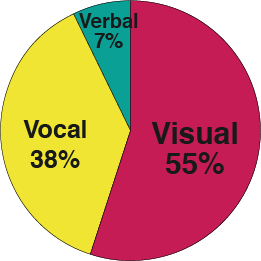
\includegraphics[width=50mm,bb=0 0 261 261]{mehrabian.jpg}}
    \end{center}
    \caption{メラビアンの法則}
    \label{fig:mehrabian}
\end{figure}


\subsection{人との繋がり形成の多様化}
直接対面でしかなかった出会いの形が,若い世代を中心に多様化している. オンライン上での出会いが増えてきている.
インターネット上で知り合った経験がある10~20代の若者世代は多い.(目的は友達になったから会う, 友達になりたくて会う, 恋人探しなど様々)
マッチングアプリなど, 自身のパートナーをインターネット上のデータを基に探すサービス展開も行われており, 登録者は1000万人を超えるものもある
結婚相手を探す新しい場を提供する,婚活パーティーも増えてきており[2],
従来の出会いの方法にくらべ敷居が低くなり,多種多様な人々との出会いの機会が提供されるようになっている.
%[20代~50代へのアンケート調査(n=1,091)で ネット上で知り合った人と直接会った割合は 10~20代で約半数
%株式会社マンダム 出会いとデジタルコミュニケーションにおける調査][1]
%[シャンクレールの調査データを使用][2]

\section{問題意識}
前章において, 人との繋がりの重要性および繋がりを形成するコミュニケーションにおける表情の重要性を述べ,
現代社会における出会いの多様性について述べた.
本節では, 本研究おける問題意識について述べる.
\subsection{情報社会における情報過多}
人との繋がり形成の場が多様化し, 出会いの入り口が広くなった分, 情報量の整理がうまくいっていない.
情報過多になっているが故に, 選択肢が多く全ての人にアプローチをして交友関係を構築することは不可能である.
ネット上の出会い調査によると若者が相手に対して残念と思った割合は〜%である.[1]
つまり, 自分の理想とする人, 自分と考えがあう人と出会える確率は現状まだ低く, また理想や考えがあう人を見逃している可能性が非常に高い.
しかし, 現状はテキストベースで判断をして自分でアプローチをかけたり, アプリケーション側で処理を行いユーザーへ情報提供をすることしかできていない.

%[20代~50代へのアンケート調査(n=1,091)で ネット上で知り合った人と直接会った割合は 10~20代で約半数
%株式会社マンダム 出会いとデジタルコミュニケーションにおける調査][1]

\subsection{相性が悪い人同士における生産性の低下}
コミュニケーションにおいて, 相手と考えが合わない場合精神的な負担が大きくなる.
Mechanic (1976) はソーシャルスキルの程度と種々の具体的問題解決能力との2側面から適応行動を規定した上で,
適応行動の不足は個体のストレスレベルを上昇させ疾患発症の危険度を高める(引用文献も明記する)
FisherBeckfield \& McFa11 (1982) は、ソーシャルスキル得点の低い男子大学生が,高い抑うつ反応を示していたと報告している.
コミュニティーにおいて考えの近い人々をグルーピングをした際にはアイスプレーキングの時間や, 相手の印象を探る時間フェーズを短くすることができ,
産出するもののクオリティーの向上や, 時間短縮を見込める.
上記のことより, 考え方の近い人や目的や嗜好が似ている人同士を引き合わせることで活動の効率化, ストレスの軽減に繋がる.
また人の考え方・内面は表情に顕著に現れると言われており, Associated Newspapers Ltd Part of the Daily Mail[2]
の調査によると目尻と口の動きは相手への信頼性を判断する材料となっている. Bruno Leangによれば, 似ている人には信頼を置きやすいと述べている.

%[https://ananweb.jp/news/246816/ ananの調査, 2019.8.28 ][1]
%[Associated Newspapers Ltd Part of the Daily Mail, The Mail on Sunday & Metro Media Group の調査][2]
%[Bruno Laeng ,Is Beauty in the Face of the Beholder?,POLOS, July 10,2013 | Volume 8 | Issue 7 ]
\subsection{断片的な表情データ}
人の表情は断片的なものではなく連続的なものである. 表情の研究は主に画像処理によって行われており,
中立の表情から笑顔になる過程については分析がほとんど行われていない.
より人間の表出表現を正確に, 繊細に分析する際には連続的に表情の流れの中で分析する必要がある.

\section{目的}
本研究の目的は, 笑顔からお互いを分析し, 人と人との繋がり作成を助長するシステムの作成である.
自身の笑い方と, 魅力を感じる笑い方にはどのような関係性があり, どの顔のパーツ・動きに由来するのかを分析する.
人の考え方・内面は表情に顕著に現れると言われており, Associated Newspapers Ltd Part of the Daily Mail[2]
の調査によると目尻と口の動きは相手への信頼性を判断する材料となっている. Bruno Leangによれば, 似ている人には信頼を置きやすいと述べている.
本研究におけるDelta Smile Facial Survey Analyzer において, ユーザーの笑顔の作り方を数値データとして取得し,
データベース内の笑顔の作り方データを表示し, 順位付けを行うことで笑顔の作り方による嗜好性を分析することが可能である.
本システムの導入により, 人と人との繋がり形成の際により最適な相手をユーザーに表示することができるようなアルゴリズムを作成することが可能になり,
ユーザーにとってよりよい出会いの機会提供を助長することができる.

%[Associated Newspapers Ltd Part of the Daily Mail, The Mail on Sunday & Metro Media Group の調査][2]
%[Bruno Laeng ,Is Beauty in the Face of the Beholder?,POLOS, July 10,2013 | Volume 8 | Issue 7 ]

\section{仮説}
人相学の分野において顔のひとつひとつの形には, その人の性格が表れるとされている.それゆえに, 顔が似ている人は性格が似ていることになる.
また心理学の分野において, Anthony Little[1]は人間同士においては特にカップルに身体的特徴, 表情が似てくる傾向があると述べている.
さらに, Robert Zajoncは実験で新婚当初に比べ結婚25年の写真ほうがお互いが似ていると結論づけている.[2]
上記の例では好意がお互いの表情を似せていることを述べている.
本研究において, 私は「表情が似ている人には好意を抱きやすい」との仮説を立てる.
William J.Chopikはか飼い主と犬の性格は似ていることを証明した[3]. 犬を迎え入れる際に人は無意識に自分の生活習慣にあった犬に惹かれる傾向があるとしている.
これは人と人との関係性にも言えることなのではないかと考えた.

%Anthony Little, Assortative mating for perceived facial personality traits,Personality and Individual Differences ,Volume 40, Issue 5, April 2006, Pages 973-984
%Robert Zajonc,Convergence in the Physical Appearance of Spouses ,Motivation and Emotion, VoL 11, No. 4, 1987
%William J.Chopik, Old dog, new tricks: Age differences in dog personality traits, associations with human personality traits, and links to important outcomes,
%Journal of Research in Personality,Volume 79, April 2019, Pages 94-108[3]


\section{本文書の構成}

本論文は, 本章を含め全7章で構成する. 本章では, 本研究における背景と問題意識, 目的および作成者の仮説を述べた.
第2章では, 関連研究をについてまとめ, 本論文における用語の意味を定義する.
第3章では, 本研究にて作成するシステムDelta Smile Facial Survey Analyzerの概要について説明をする.
第4章では, 本システムにおける設計について整理する.
第5章では, 本システムの実装について述べる.
第6章では, 予備実験について述べる.
第7章では, データ収集および評価実験について述べる.
第8章では, 結論および今後の展望について述べる.
%chapであとで管理

第\ref{chap:introduction}章では本テンプレートの概要みたいなものを書いた。第\ref{chap:howto}章では、本テンプレートの使い方を説明する。第\ref{chap:latex}章で図表や数式の挿入など代表的な\LaTeX コマンドを解説する。第\ref{chap:conclusion}章では、『序論』で始めたら『結論』で終われと書いた手前書かざるを得ないので、なにか結論らしいことを書く。付録として、テンプレートのサンプルになるように無理矢理ゴミを添付する。
